\documentclass{csc_assignment}
\usepackage[utf8]{inputenc}
\usepackage[letterpaper, portrait, margin=1in]{geometry}
\usepackage{calc}  % arithmetic in length parameters
\usepackage{enumitem}  % more control over list formatting
\usepackage{fancyhdr}  % simpler headers and footers
\usepackage{lastpage}  % for last page number
\usepackage{relsize}  % easier font size changes
\usepackage[normalem]{ulem}  % smarter underlining
\usepackage{url}  % verb-like typesetting of URLs
\usepackage{xfrac}  % nicer looking simple fractions for text and math
\usepackage{amsmath}
\usepackage{amssymb}
\usepackage{tikz}
\usepackage{algorithm}
\usepackage{algorithmic}
\usepackage{graphicx}
\usepackage{lipsum}
\graphicspath{{/}}

% ----------------------------------------------------------------
% TODO: Enter the assignment number, your name, and your student number below
% ----------------------------------------------------------------
\AssignmentName{Problem Set 1}
\StudentName{Akhil Gupta}
\StudentNumber{1000357071}

% ----------------------------------------------------------------
\begin{document}
\begin{description}

\item[Q1.]
Suppose we have the following two-dimensional matrix to be sent: \\\\
\begin{tabular}{ |ccccccc|c| }
\hline
	\multicolumn{7}{|c|}{Data} & Parity Bit \\
	\hline
	0 & 1 & 0 & 0 & 1 & 0 & 1 & 1 \\
	1 & 0 & 0 & 1 & 0 & 0 & 1 & 1 \\
	0 & 1 & 0 & 1 & 0 & 1 & 1 & 0 \\
	1 & 0 & 0 & 0 & 0 & 0 & 1 & 0 \\
	\hline
	0 & 0 & 0 & 0 & 1 & 1 & 0 &   \\
\hline
\end{tabular} \\

and we receive the following two-dimensional matrix: \\\\
\begin{tabular}{ |ccccccc|c| }
\hline
	\multicolumn{7}{|c|}{Data} & Parity Bit \\
	\hline
	0 & 1 & 0 & 0 & 1 & 0 & 1 & 1 \\
	1 & 0 & 0 & 1 & 0 & 0 & \textbf{0} & \textbf{0} \\
	0 & 1 & 0 & 1 & 0 & 1 & 1 & 0 \\
	1 & 0 & 0 & 0 & 0 & 0 & 1 & 0 \\
	\hline
	0 & 0 & 0 & 0 & 1 & 1 & \textbf{1} &   \\
\hline
\end{tabular} \\

We can see that there is an error in row 2, column 7 of the data (shown in bold), which in turn will change the row and column parity bit. Thus, by looking at the intersection of the row and column parity bit, we can easily detect as well as correct a single bit error. \\ To show that double-bit error can be detected but not corrected, we will use the same two-dimensional matrix we sent, but change 2 bits in the received matrix; namely row 2, column 7 \& row 3, column 7.  \\\\
\begin{tabular}{ |ccccccc|c| }
\hline
	\multicolumn{7}{|c|}{Data} & Parity Bit \\
	\hline
	0 & 1 & 0 & 0 & 1 & 0 & 1 & 1 \\
	1 & 0 & 0 & 1 & 0 & 0 & \textbf{0} & \textbf{0} \\
	0 & 1 & 0 & 1 & 0 & 1 & \textbf{\underline{0}} & \textbf{\underline{1}} \\
	1 & 0 & 0 & 0 & 0 & 0 & 1 & 0 \\
	\hline
	0 & 0 & 0 & 0 & 1 & 1 & \textbf{\underline{0}} &   \\
\hline
\end{tabular} \\

Now we see that the row and column parity bits have changed again (show in bold underline), but this time we cannot pin-point the exact location of the error bits since the 7th column in the data had 0 parity bit when we sent it, and after receiving the data with errors, we still have the 7th column with a 0 parity bit. Hence, we will be unable to locate which column has the error, but we can locate which row has the error. 

% ----------------------------------------------------------------
% Answer ends
% ----------------------------------------------------------------

\item[Q2.]
  \begin{enumerate}
  \item No, E will not perform an ARP query to find B's MAC address because they are not connected on the same LAN. We send an Ethernet frame (destined to B) from E to Router R1: \\
  Source IP Address: E's IP Address \\
  Destination IP Address: B's IP Address \\
  Source MAC Address: E's MAC Address \\
  Destination MAC Address: R1's MAC Address of interface that connects to Subnet 3
  \item Once switch S1 receives the ARP request message from A it will broadcast it both its interfaces, i.e. to router R1's interface that connects to Subnet 2. Also, S1 creates an entry as it learns that Host A is on S1's interface that connects it to Subnet 1. Yes, router R1 will also receive this ARP request but it will not forward the message to Subnet 3. No, Host B will not send an ARP query message to ask for A's MAC address because this address can be deciphered from A's query message. Once switch S1 receives an ARP response message from Host B, it will not add it to its forwarding table as it is already present (given in question), then it will drop the received message as destination Host A is on the same LAN segment as Host B. 
  \end{enumerate} 
  
% ----------------------------------------------------------------
% Answer ends
% ----------------------------------------------------------------

\item[Q3.]
	\begin{enumerate}
	\item The minimum RTT for the link is twice the time taken for data to travel from Earth to Moon = 
	$\frac{385,000*1000}{3*10^8}$ = $1.284s * 2 = 2.568s$
	\item Delay x Bandwidth Product = $2.568s * 1Gbps = 2.568Gb = 2568000000 bits$
	\item Delay x Bandwidth Product tells us the measure of ``data in flight'' i.e. it tells us how much data can be sent before the receiver sees any of it
	\item Firstly, the request to download the most current image from Earth to Moon will take $1.284s$. Then, the time to load the image onto the link is 
	$\frac{25MB}{1Gbps} = \frac{25*1024*1024*8}{1Gbps} = \frac{209,715,200bits}{10^{9}bits/s} = 0.21s.$ Then, it will take another $1.284s$ for the image to return to Earth. Therefore, the minimum amount of time that will elapse = $1.284 + 0.21 + 1.284 = 2.778s$
	\end{enumerate}
  
% ----------------------------------------------------------------
% Answer ends
% ----------------------------------------------------------------

\item[Q4.]
	\begin{enumerate}
	\item The latency = Transmit Time + Propagation Delay. To calculate transmit time, we need to calculate the time it takes to put 12,000 bits onto a 100-Mbps link = \\
	$\frac{12,000}{100*10^{6}}$ = $\frac{12,000}{10^{8}}$ = $0.0012s$ = $1.2ms$. Then we add the propagation delay = $1.2ms + 0.01ms$ = $1.21ms$. It takes another $1.21ms$ for the switch to send the packet to the destination and destination to receive till the last bit, therefore, total latency = $2*1.21ms=2.42ms$.
	\item Now we have 3 switches, which means we have 4 links. From $(a)$, we know that each link takes $1.21ms$, therefore, total latency with 3 switches = $4*1.21ms=4.84ms$.
	\item First we have to calculate the time it would take to send the first 200 bits: \\
	      $\frac{200}{100*10^{6}}$ = $\frac{200}{10^{8}}$ = $0.000002s$ = $0.002ms$. Then we add the propagation delay = $0.002ms + 0.01ms$ = $0.012ms$. It takes another $1.21ms$ for the switch to send the packet to the destination and another $0.01ms$ for the destination to receive the entire packet. Hence, total latency = $0.012ms + 1.21ms + 0.01ms = 1.232ms$.
	\end{enumerate}

% ----------------------------------------------------------------
% Answer ends
% ----------------------------------------------------------------

\item[Q5.]
The NRZ, Manchester and NRZI encodings are shown below: 
\begin{figure}[h]
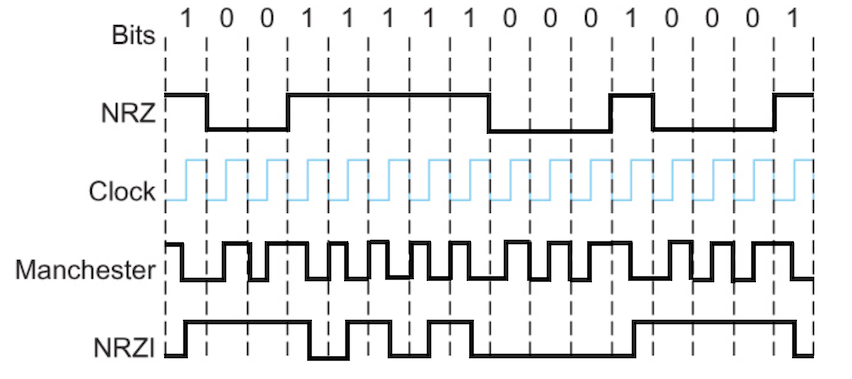
\includegraphics[scale=0.75]{358.png}
\vspace{-50mm}
\end{figure}
% ----------------------------------------------------------------
% Answer ends
% ----------------------------------------------------------------

\newpage
\item[Q6.]
\begin{enumerate}
\item The long division is shown below: \\
Message: 11100011; Generator: 1001; So we divide 11100011\textbf{000} by 1001\\
Remainder: 111; Message to be sent: 11100011\textbf{111}
\[\setlength{\arraycolsep}{0pt}
\begin{array}[t]{*{16}{l}}
	&1&1&1&0&0&0&1&1&0&0&0\\
	1&0&0&1\\ \cline{1-4}
	&1&0&1&0\\
	&1&0&0&1&&&&&&&&&&&\\\cline{2-5}
	&&0&0&1&0&&&&&&&&&&\\
	&&0&0&0&0&&&&&&&&&&\\\cline{3-6}
	&&&0&1&0&1&&&&&&&&&\\
	&&&0&0&0&0&&&&&&&&&\\\cline{4-7}
	&&&&&1&0&1&1&&&&&&&\\
	&&&&&1&0&0&1&&&&&&&\\\cline{6-9}
	&&&&&&&0&1&0&0&&&&&\\
	&&&&&&&0&0&0&0&&&&&\\\cline{8-11}
	&&&&&&&&1&0&0&0&&&&\\
	&&&&&&&&0&0&0&0&&&&\\\cline{9-12}
	&&&&&&&&1&0&0&0&0&&&\\
	&&&&&&&&&1&0&0&1\\\cline{10-16}
	&&&&&&&&&0&1&1&1&&&\\
\end{array}/1001=11001001
\]
\item The received message is \textbf{0}1100011111. The receiver then divides the message by 1001.
\[\setlength{\arraycolsep}{0pt}
\begin{array}[t]{*{16}{l}}
	&0&1&1&0&0&0&1&1&1&1&1\\
	0&0&0&0\\ \cline{1-4}
	&1&1&0&0\\
	&1&0&0&1&&&&&&&&&&&\\\cline{2-5}
	&&0&1&1&0&&&&&&&&&&\\
	&&0&0&0&0&&&&&&&&&&\\\cline{3-6}
	&&&1&1&0&1&&&&&&&&&\\
	&&&1&0&0&1&&&&&&&&&\\\cline{4-7}
	&&&&&1&0&0&1&&&&&&&\\
	&&&&&1&0&0&1&&&&&&&\\\cline{6-9}
	&&&&&&&0&0&0&1&&&&&\\
	&&&&&&&0&0&0&0&&&&&\\\cline{8-11}
	&&&&&&&&0&0&1&1&&&&\\
	&&&&&&&&0&0&0&0&&&\\\cline{9-12}
	&&&&&&&&&0&1&1&1&&&\\
	&&&&&&&&&0&0&0&0\\\cline{10-16}
	&&&&&&&&&0&1&1&1&&&\\
\end{array}/1001=01011000
\]
We get a quotient of 01011000 and remainder of 111 $\neq$ 0. Hence, the receiver knows that an error has occured.
\end{enumerate}

% ----------------------------------------------------------------
% Answer ends
% ----------------------------------------------------------------

\newpage
\item[Q7.]
The datagram forwarding table is given below: \\\\
\begin{tabular}{ |c|c|c| }
\hline
	Node & Destination & Next Hop \\
	\hline
	A & A & - \\
	A & B & C \\
	A & C & C \\
	A & D & C \\
	A & E & C \\
	A & F & C \\
	\hline
	B & A & E \\
	B & B & - \\
	B & C & E \\
	B & D & E \\
	B & E & E \\
	B & F & E \\
	\hline
	C & A & A \\
	C & B & E \\
	C & C & - \\
	C & D & E \\
	C & E & E \\
	C & F & F \\
	\hline
	D & A & E \\
	D & B & E \\
	D & C & E \\
	D & D & - \\
	D & E & E \\
	D & F & E \\
	\hline
	E & A & C \\
	E & B & B \\
	E & C & C \\
	E & D & D \\
	E & E & - \\
	E & F & C \\
	\hline
	F & A & C \\
	F & B & C \\
	F & C & C \\
	F & D & C \\
	F & E & C \\
	F & F & - \\
	\hline
\end{tabular} \\

% ----------------------------------------------------------------
% Answer ends
% ----------------------------------------------------------------

\item[Q8.]
The ports that are not selected by the spanning tree algorithm are: B2 - A, B5 - B, B5 - F and B6 - I. B2 - A because B7 is closer to the root than B2. B5 - B because B2 is closer and has lower ID. B5 - F because B3 is closer to the root. B6 - I because B4 has equal distance but lower ID.

% ----------------------------------------------------------------
% Answer ends
% ----------------------------------------------------------------

\item[Q9.]
\begin{enumerate}
\item All three bridges B1, B2 and B3 learn the location of X. Yes, Y's network interface does see this packet as bridge B2 floods the packet it receives on all its interfaces. 
\item All three bridges B1, B2 and B3 learn the location of Z. No, Y's network interface does not see this packet as bridge B2 learnt the location of X and knows where to forward the packet.
\item Only bridges B1 and B2 learn the location of Y. No, Z's network interface does not see this packet as B2 did not forward it to B3 because B2 knows the location of X.
\item Only bridges B2 and B3 learn the location of W. Yes, Z's network interface does see this packet as B3 does not know the location of Y so it floods on all its interfaces. 
\end{enumerate}

% ----------------------------------------------------------------
% Answer ends
% ----------------------------------------------------------------

\item[Q10].
We have a class C which means we can have a maximum of $2^{8}$ = 256 hosts. Our organization requires 148 hosts in total divided amongst 4 departments. 
\begin{enumerate}
\item
\begin{tabular}{ |c|c|c|c|c|c|c| }
\hline
	Subnet \# & Department & Hosts & Max Hosts & Network ID & Subnet Mask & IP Addresses \\
	\hline
	1 & A & 75 & 128 & 212.1.1.0 & 255.255.255.128 & 212.1.1.0 - 212.1.1.127 \\
	\hline
	2 & B & 35 & 64 & 212.1.1.128 & 255.255.255.192 & 212.1.1.128 - 212.1.1.191 \\
	\hline
	3 & C & 20 & 32 & 212.1.1.192 & 255.255.255.224 & 212.1.1.192 - 212.1.1.223 \\
	\hline
	4 & D & 18 & 32 & 212.1.1.224 & 255.255.255.224 & 212.1.1.224 - 212.1.1.255 \\
	\hline
\end{tabular} \\

\item If department D grows to 32 hosts, we could split subnet \#1 (department A) into 3 subnets. 2 of those 3 would have 32 hosts each, and the third one would have 64 hosts. So, we would have A1 = 64 hosts, A2 = 32 hosts and A3 = 32 hosts. Then, we could allocate A3 to department D so they would have 32 + 32 = 64 hosts. \\\\
\begin{tabular}{ |c|c|c|c|c|c|c| }
\hline
	Subnet \# & Department & Hosts & Max Hosts & Network ID & Subnet Mask & IP Addresses \\
	\hline
	1A & A & Total & 64 & 212.1.1.0 & 255.255.255.192 & 212.1.1.0 - 212.1.1.63 \\
	1B & A & 75 & 32 & 212.1.1.64 & 255.255.255.224 & 212.1.1.64 - 212.1.1.95 \\
	\hline
	2 & B & 35 & 64 & 212.1.1.128 & 255.255.255.192 & 212.1.1.128 - 212.1.1.191 \\
	\hline
	3 & C & 20 & 32 & 212.1.1.192 & 255.255.255.224 & 212.1.1.192 - 212.1.1.223 \\
	\hline
	4A & D & Total & 32 & 212.1.1.96 & 255.255.255.224 & 212.1.1.96 - 212.1.1.127 \\
	4B & D &  32 & 32 & 212.1.1.224 & 255.255.255.224 & 212.1.1.224 - 212.1.1.255 \\
	\hline
\end{tabular} \\
\end{enumerate}

% ----------------------------------------------------------------
% Answer ends
% ----------------------------------------------------------------

\item[Q11.]
Applying a subnet mask means performing a bit-wise $and$ with the incoming packet to get the subnet number. The router applies both the subnet masks (255.255.254.0 and 255.255.252.0) and chooses the subnet number using longest prefix match.
\begin{enumerate}
\item 128.96.171.92: router applies subnet mask 255.255.254.0 to 128.96.171.92. We get 128.96.170.0. router applies subnet mask 255.255.252.0 to 128.96.171.92. We get 128.96.168.0. Since 128.96.170.0 has a longer prefix, the router forwards the packet on its interface 0.
 
\item 128.96.167.151: router applies subnet mask 255.255.254.0 to 128.96.167.151. We get 128.96.166.0. router applies subnet mask 255.255.252.0 to 128.96.171.92. We get 128.96.164.0. Since 128.96.166.0 has a longer prefix, the router forwards the packet to R2. 

\item 128.96.163.151: router applies subnet mask 255.255.254.0 to 128.96.163.151. We get 128.96.162.0. router applies subnet mask 255.255.252.0 to 128.96.163.151. We get 128.96.160.0. Since none of the subnet numbers match, the router uses default router R4. 

\item 128.96.169.192: router applies subnet mask 255.255.254.0 to 128.96.169.192. We get 128.96.168.0. router applies subnet mask 255.255.252.0 to 128.96.169.192. We get 128.96.168.0. Since both have the same subnet number, the router forwards the packet on its interface 1.  

\item 128.96.165.121: router applies subnet mask 255.255.254.0 to 128.96.165.121. We get 128.96.164.0. router applies subnet mask 255.255.252.0 to 128.96.165.121. We get 128.96.164.0. Since both have the same subnet number, the router forwards the packet to R3.

% ----------------------------------------------------------------
% Answer ends
% ----------------------------------------------------------------

\item[Q12.]  
If two hosts on the same Ethernet share the same hardware address i.e. MAC Address, it could lead to quite some problems. First, the Address Resolution Protocol (ARP) will cause some trouble as it is used to distinguish individual computers' MAC Address. So, ARP will not be able to correctly identify which host to send the packet to. As a result, the packet could be delivered to the wrong host which could potentially harm the host. Also, if the hosts share a switch on the Ethernet line, a switch maintains a forwarding table based on MAC addresses, so the switch will continuously update the address table leading to undesired behaviour. 

\end{enumerate}

\end{description}
\end{document}
  
  



